\chapter{Maxwell's Equations.}
	\section{Introduction}
	In the last lecture, the mathematical equations of the physical laws of electromagnetism were established these laws include; ampere's circuit law, gauss law, Faraday's law of electromagnetic induction. Compiling these laws in mathematical form gives \textbf{'Maxwell's Equations'}, and this compilation was done by Maxwell. In compiling these laws Maxwell discovered some inconsistency in the ampere's circuit law. This inconsistency was examined and modified. This  would be discussed shortly.
	\section{Ampere Circuit Law Modification and the 'Maxwell's Equations'}
	\begin{figure}[h]
		\centering
		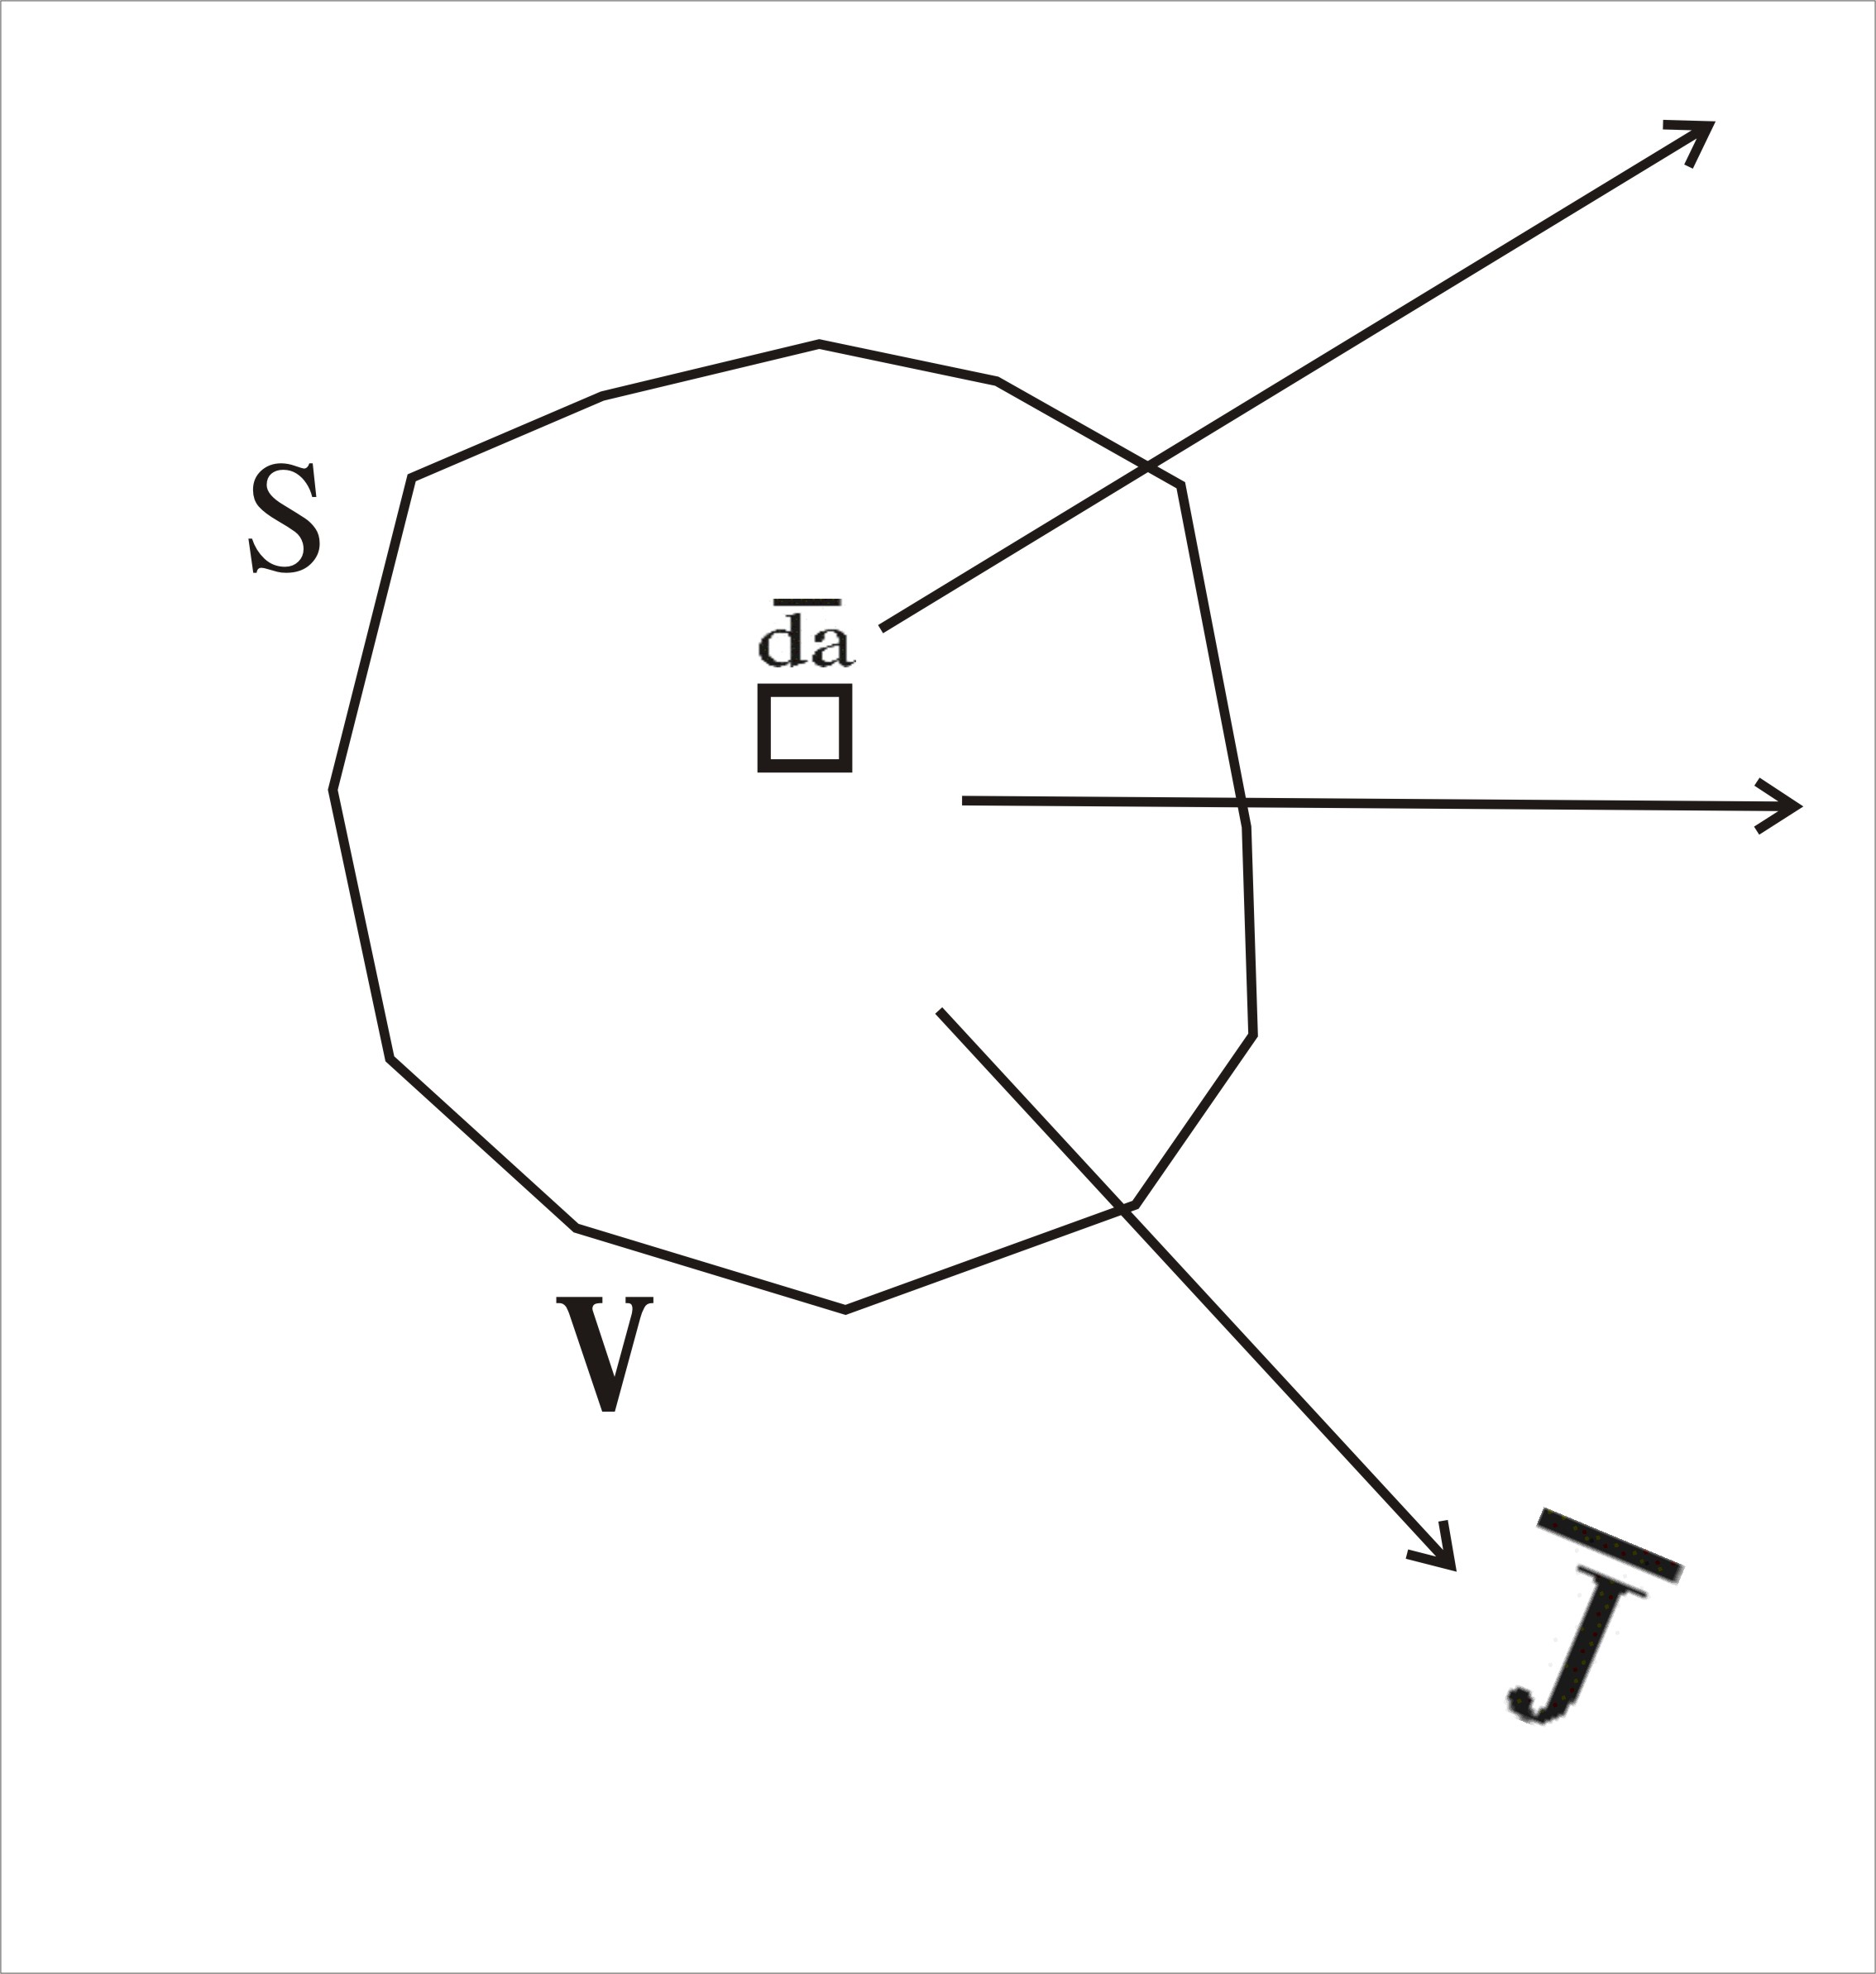
\includegraphics[height=5cm]{closedsurface}
		\caption{\textbf{Conduction current density from a closed surface}}
	\end{figure}
 
 
 
 Consider a closed surface S of certain volume V shown in figure 19.1. Assuming the charges are distributed inside the surface, there is the possibility that the charges would leave from the surface and when this happens, there would be a rate of change of charge. This means there will be current flow from the surface and hence a current density is distributed on the surface. The charges would leave in the form of current leading to a reduction in the net charge inside the surface.
 
 
 The concept of charge-current relation has been has been worked out and it also applied to the closed surface in figure 19.1. The current produced on the surface would yield a surface current density.This current density is the vector field around the surface. Lets say we denote this current density of the surface with $\bar{J}$. If we take the divergence of $\bar{J}$, it would stand for the outflow of the electric vector field($\bar{J}$).
 
 
 If we consider a small area on the closed surface S given by $\bar{da}$. Then the product of conduction current density $\bar{J}$ and the small area  $\bar{da}$ gives the outward current from the infinitesimally small area  $\bar{da}$. By summing over the entire surface(basically integrating), then we get the net outward current flow from the whole surface S. \\\\
\begin{align}
\textbf{Net outward current}= \oiint\limits_S\bar{J}\cdot\bar{da}
\end{align},
 but as we know current is actually rate of change of charge and since this current is coming out from the surface, it should be equal to rate of charge from the total volume and since the current is coming outwards, the net charge must be decreasing inside the volume. So if the volume is said to have a charge density denoted by $\rho C/m^{3}$, then the net decrease or the rate of change of decrease of charge inside the volume is the same as the total current coming out from the surface.  To get the total charge enclosed by the closed surface S, we get the integral of $\rho$ over the volume created by the closed surface.\\
	\begin{align}
\textbf{rate of charge decrease in volume}	= -\frac{\partial}{\partial t}\iiint \rho dv
	\end{align}
	\\ So we get that;
	\begin{align}
	\oiint\limits_S\bar{J}\cdot\bar{da} =  -\frac{\partial}{\partial t}\iiint\limits_V\rho dv
	\end{align}
	\\ If we say volume is not changing with time, so that it is only $\rho$ that  changes with time, we have that;
	\begin{align}
	\oiint\limits_S\bar{J}\cdot\bar{da} = -\iiint\limits_V\frac{\partial\rho}{\partial t}dv
		\end{align}
	 We can convert surface integral to volume integral by  using divergence theorem. Establishing this, we get that;
	\begin{align}
		\oiint\limits_S\bar{J}\cdot\bar{da} = \iiint\limits_V(\nabla\cdot\bar{J})dv
	\end{align}
	\\ from this we get that;
	\begin{align}
	\iiint\limits_V(\nabla\cdot\bar{J})dv = -\iiint\limits_V\frac{\partial\rho}{\partial t}dv
	\end{align}
  this would give;
  \begin{align}
  \iiint\limits_V(\nabla\cdot\bar{J} + \frac{\partial\rho}{\partial t} )dv = 0
  \end{align}
  and since this relation we have gotten in equation 19.7 should be true for any arbitrary volume, so the integral must be zero, so we get;
  \begin{align}
  \nabla\cdot\bar{J} = -\frac{\partial\rho}{\partial t}
  \end{align}
  this is called \textbf{Continuity Equation}, this should be duly noted.
  
  
  So if we have time varying charges, the $-\frac{\partial\rho}{\partial\rho}$ is a finite quantity and divergence of the conduction current density $\nabla\cdot\bar{J}$ is not zero. But if we take a case where the charges are not varying that is a static case, then the rate of change of charge will be zero $(\frac{\partial\rho}{\partial\rho}=0)$ and so $\nabla\cdot\bar{J}=0$. This makes makes physical sense, especially when looking at it with the concept of divergence, which as we know measures the net quantity coming out from a unit volume, and since $(\frac{\partial\rho}{\partial\rho}=0)$, there would be no net flow and thus no divergence. So if current is coming out from this volume it means that surface charge must be leaving the volume, then there must be a change in the total charge or change in charge density inside the volume.
  
  
  If the charges are not changing inside the volume(static case), then whatever charge entering the volume is the same as charge leaving the volume. So the net charge inside the volume is the same and in that case the divergence of the conduction current is zero. So whenever we have 'time varying quantities', the continuity equation must be satisfied by the conduction current density and the charges. This 'continuity equation' was what led to the difficulty in compiling other equations by maxwell. Now let us examine this difficulty.
  
  
  We had earlier seen from the previous chapter, that from Ampere's circuit law we get the relation $\nabla\times\bar{H}=\bar{J}$, that is the curl of the magnetic field is equal too the conduction current density. If we apply vector operation on this without taking note of the physical aspects( that is the physical meaning of $\nabla\times and  \nabla\cdot$), we can expand both sides of the 'Ampere's circuit law' relation to get;
  \begin{align}
  \nabla\cdot(\nabla\times\bar{H})=\nabla\cdot\bar{J}
  \end{align}
  knowing that we can interchange $\nabla\times and  \nabla\cdot$ then the relation becomes;
  \begin{align}
  \nabla\times(\nabla\cdot\bar{H})=\nabla\cdot\bar{J}
  \end{align}
  but $\nabla\times\nabla\cdot\bar{H}$ is actually zero by identification. This imply that $\nabla\cdot\bar{J}=0$. So from Ampere's circuit law $\nabla\cdot\bar{J}=0$ while for the ' continuity equation'  $\nabla\cdot\bar{J}=-\frac{\partial\rho}{\partial t}$.
  
  
  The inconsistency arise from the fact that Ampere's circuit law does not satisfy the continuity equation. This was the difficulty that was encountered by Maxwell. He resolved this difficulty  by introducing the concept of the '\textbf{Displacement Current Density}'. So what he said was that "in the continuity relation $\nabla\cdot\bar{J}=-\frac{\partial\rho}{\partial t}$ replace $\rho$ from Gauss law with divergence of displacement vector $\bar{D}$", that is $\rho=\nabla\cdot\bar{D}$. So we have;
  \begin{align}
  \nabla\cdot\bar{J}=-\frac{\partial}{\partial t}(\nabla\cdot\bar{D})
  \end{align}
  Interchanging space and time operators, we have;
  \begin{align}
  \nabla\cdot\bar{J}=-\nabla\cdot(\frac{\partial\bar{D}}{\partial t}) \\ 
  \nabla\cdot\bar{J}+\nabla\cdot(\frac{\partial\bar{D}}{\partial t})
  \end{align}
  we then integrate over the entire volume of the closed surface to get;
    \begin{align}
    \iiint\limits_V\nabla\cdot\bar{J}+\nabla\cdot(\frac{\partial\bar{D}}{\partial t})dv=
     \oiint\limits_S(\bar{J}+\frac{\partial\bar{D}}{\partial t})=0
    \end{align}
   Equation 19.4 is gotten by divergence theorem
    
  This surface integral implies that the current which is coming from the closed surface S, is not only because of the 'conduction current density' $\bar{J}$, but also as  result of $\frac{\partial\bar{D}}{\partial t}$ which is the 'Displacement Current Density' So for a homogenous equation $\frac{\partial\bar{D}}{\partial t}$ has the same unit as current density. However Displacement Current Density does not depend on the conductivity of the medium unlike conduction current density $\bar{J}$ that does. $\bar{J}$ is related conductivity by ohms law $\bar{J}=\sigma\bar{E}$. However if $\sigma=0$, then we have only $\frac{\partial\bar{D}}{\partial t}$ from $\bar{J}+\frac{\partial\bar{D}}{\partial t}$ to play with. The quantity $\frac{\partial\bar{D}}{\partial t}$ is equal to some current and hence it is called Displacement Current Density. So $\frac{\partial\bar{D}}{\partial t}$ is the quantity that was introduced by maxwell to satisfy the 'continuity equation'.
  
  
  So the net current from any closed surface is not only due to conduction current density $\bar{J}$ alone, but the summation of $\bar{J}$ and the 'displacement current density' $\frac{\partial\bar{D}}{\partial t}$. So if we use this summation to define the total current, then Ampere's law can be modified to say that " 
  \textbf{The Magnetomotive Force around a closed loop is equal to the total current enclosed by that loop which includes the conduction current as well as displacement current}". It should be noted that current due to displacement current density is not due to charge flow, infact it can exist without the presence of charges(and hence conduction current density $\bar{J}$). $\frac{\partial\bar{D}}{\partial t}$ is related to electric field $\bar{E}$. So even without charges, if we have electric field that is time varying, $\frac{\partial\bar{D}}{\partial t}$ will equate to a current flow. So the quantity $\frac{\partial\bar{D}}{\partial t}$ represent the rate of charge of electric field and this is essentially current.
  
  
  So if we take the total current which is a combination of conduction current and displacement current, this would give the $magnetomotive force$ around a closed loop.
  Ampere's circuit law is thus modified with current being the sum of conduction current and displacement current.\\
  Amperes law is modified to;
  \begin{align}
 \nabla\times\bar{H}=\bar{J}+\frac{\partial\bar{D}}{\partial t}
 \end{align}
  
  
 This essentially resolves the difficulty which was faced by Maxwell and this gives the complete description of the phenomenon of electro-magnetics. With these equations which we have gotten so far (that is gauss law of magnetic field, Faraday's law of electromagnetic induction and the modified amperes law), we have a complete set of equations which represent the static and time varying electric and magnetic fields. These equations are called \textbf{Maxwell's Equations}.As we earlier mentioned, Maxwell's equations can be written in differential form or in integral form and depending on the suitability, the equations can be used in either form. Finally we make a list for the four Maxwell's Equation.
 
 \begin{table}[h]
 	\caption{\textbf{Maxwell's Equations}}
 	\centering
 	\begin{tabular}{p{3cm} p{2cm} p{2cm}}
 		\hline \\
 		\textbf{Electromagnetic Laws} & \textbf{Differential form} & \textbf{Integral form} \\ [0.5ex]
 		\hline \\
 		Gauss laws; & $\nabla\cdot\bar{D}=\rho$ & $\oiint\limits_S\bar{D}\cdot\bar{da}=\iiint\limits_V
 		\rho dv$\\
 		 & $\nabla\cdot\bar{B}=0$ & $\oiint\limits_S\bar{B}\bar{da}=0$\\
 		 \hline \\
 		 
 		 Faradays law; & $\nabla\times\bar{E}=-\frac{\partial\bar{B}}{\partial t}$ & $\oint\limits_C\bar{E}\cdot\bar{dl}=-\iint\limits_S\frac{\partial\bar{D}}{\partial t}\cdot\bar{da}$ \\
 		 \hline \\
 		 Modified Amperes Law; &
 		 $\nabla\times\bar{H}=\bar{J}+\frac{\partial\bar{D}}{\partial t}$ & $\oint\limits_C\bar{H}\bar{dl}=\iint\limits_S(\bar{J}+\frac{\partial\bar{D}}{\partial t})\cdot\bar{da}$ \\
 		 \hline
 	 	\end{tabular}
 \end{table}


These are the set of equations which governs the total phenomenon of electro-magnetics for $static$ as well as $time$ $varying$ $fields$ so once we have these generalized equations, we can reduce the equation to get those for $Static$ $Fields$ by putting all time derivatives to zero. So depending on whether the 'medium parameter' (permeability $\mu$,permit $\epsilon$) of the medium is varying as a function of space(inhomogeneous) or is constant as a function of space (homogeneous), we can get $\bar{D}=\epsilon\bar{E}$ and $\bar{B}=\mu\bar{H}$. So we cn have various forms of these equations depending upon the condition applied to the medium; whether we are dealing with given electric fields, magnetic fields, or whatever parameters associated with them. As we said,for static fields, the time varying parameters become zero. Looking at Table 19.1, it essentially means that the equations with time derivatives become; $\nabla\times\bar{E}=0$ and $\nabla\times\bar{H}=\bar{J}$.
;

However in this part of the course, which is on Electromagnetic Waves, we are dealing with time varying quantities only, and so all the quantities ($\rho,\bar{B},\bar{J},\bar{H}$ and so on), will be considered as time varying. Later on, we will look for solution to these equations of time varying fields.


As we mentioned earlier the Maxwell's equations in differential form cannot be applied in a certain situation where a medium has discontinuity. That means if we talk about media interfaces where medium properties suddenly change, like permitivity or permeability suddenly change, at those boundaries of abrupt change the derivatives cannot be defined. So the differential form of Maxwell's equations is not useful in this situation. However, as we have mentioned the integral form is always useful and can be applied in any situation. However, if we apply the integral form to discrete media interfaces, we get relationships between the quantities $\bar{D}, \bar{B}, \bar{E}, \bar{H}$ in the two media just across the interface. That relationship is what we call the \textbf{Boundary Condition}. The same set of equations in differential form gives what is called $Point$ $Relation$ that is they are valid at every point in space. The equation in integral form when applied to discrete media interfaces gives what is called $Boundary$ $Condition$. However before we go into boundary condition, we will introduce the concept of surface current and surface charges.
\\
 \section{Concept of Surface Charges and Surface Current}
 \begin{figure}[h]
 	\centering
 	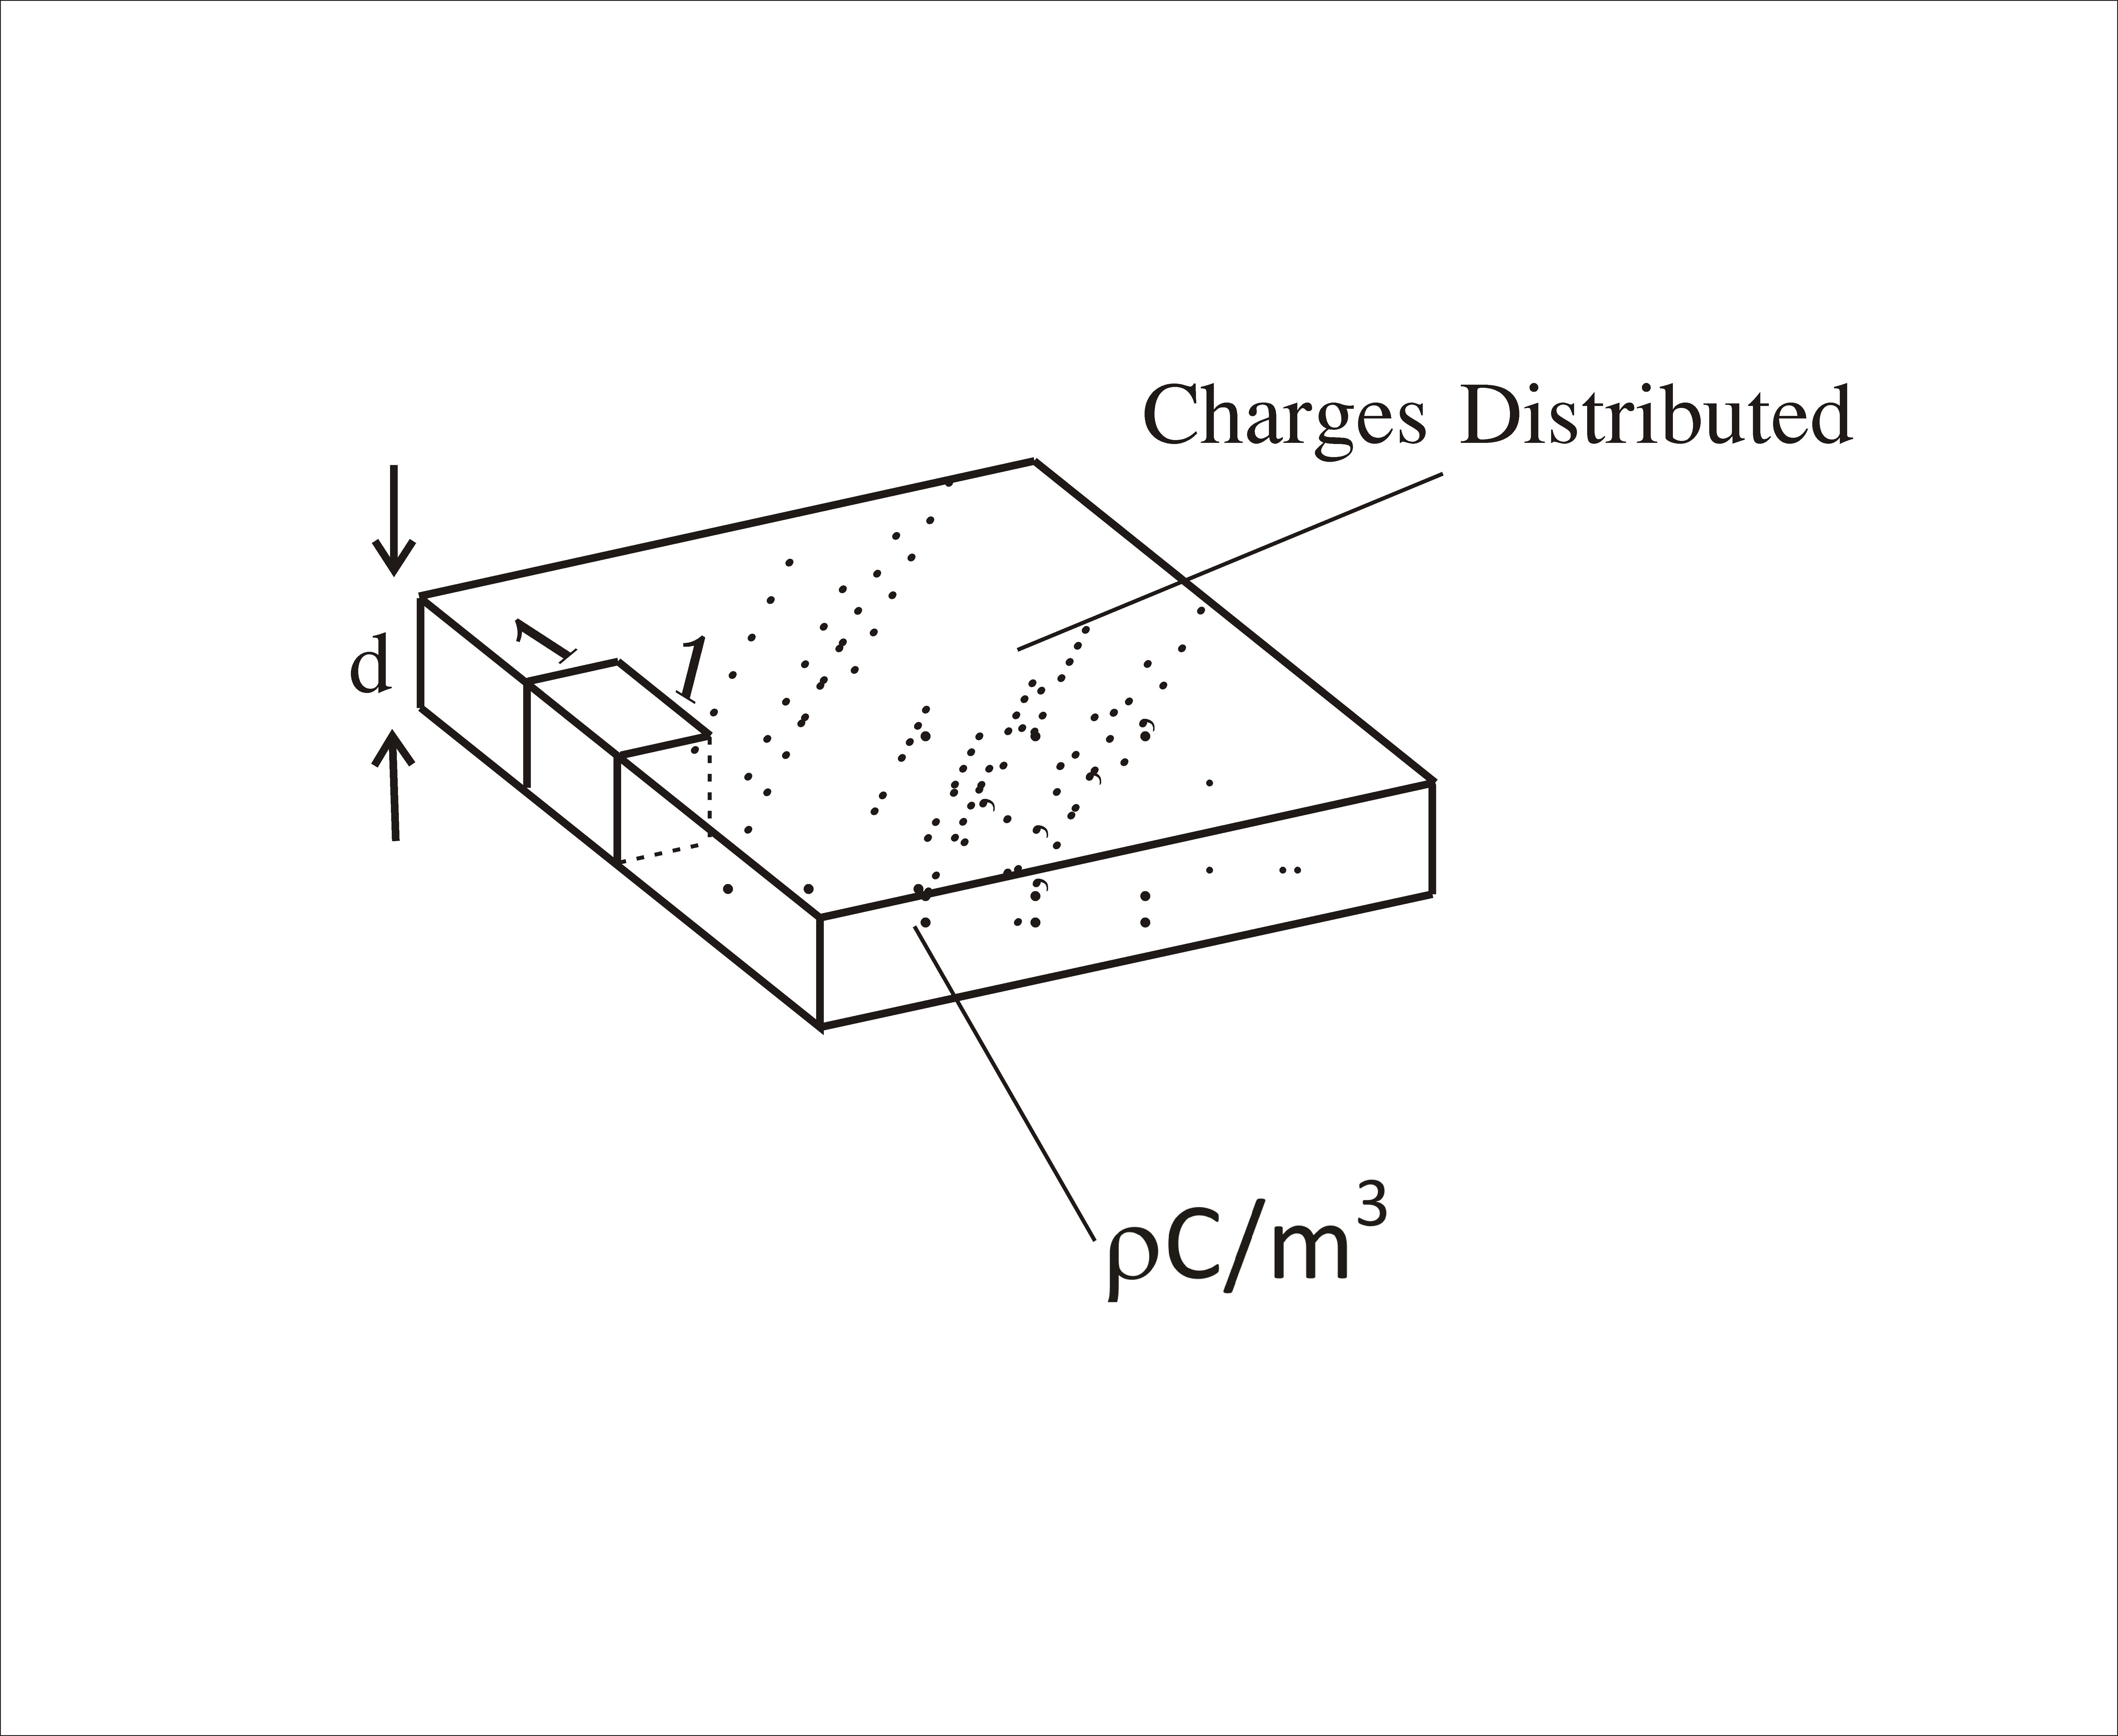
\includegraphics[width=1\linewidth]{surfacecharge}
 	\caption{\textbf{Model for studying surface charge}}
 \end{figure} 
\subsection{Surface Charge and Surface Charge Density}
Let us look at a surface with thickness d, and a charge density $\rho$$C/m^{3}$ as shown in figure 19.2, considering  unit area on the surface, with length 1 and width 1. So if a volume of unit area on the surface of the sheet is considered, the total charge which which will be in this volume which is having a height d and area 1, is the charge density $\rho$ multiplied by the elemental volume.\\
Total charge in unit volume of slab is;
\begin{align*}
=\rho\times(1\times 1\times d)=\rho d
\end{align*}
 the unit is Coulombs C.
 
 
 If we now reduce the thickness of this slab, and go to a limit when \textbf{d} tends to zero ($d\rightarrow 0$), then as a result, current density would tend to infinity ($\rho\rightarrow\infty$), so that the product '$\rho d$' would tends to finite quantity. in this situation ($d\rightarrow 0$, $\rho\rightarrow\infty$), we see a net charge which is just on the surface because the charge is now confined to a thickness of zero. This essentially implies the charge will just be lying on the surface and that charge is in the unit area. 
 
 
 So if we take the quantity $\rho d$ and take the limit when $d\rightarrow0$, we get a quantity which is charge distributed on the surface and thus there would be a charge density confined on the surface. The unit for $surface$ $charge$ $density$ $\rho_{s}$ is actually $C/m^{2}$ unlike $volume$ $charge$ $density$ $\rho$ ($C/m^{3}$).\\
 So we say that;
 \begin{align}
 \rho_{s}=\lim_{d\rightarrow0}\{\rho d\} 
 \end{align}
 This relation is called \textbf{Surface Charge Density}.
 
 
 So two things we note here, if we go from volume charge density $\rho$ to surface charge density $\rho_{s}$, when $d\rightarrow0$, the surface charge density $\rho_{s}$ is equal to infinite volume charge density($\rho\rightarrow\infty$). If that infinite volume charge density is confined to our thickness, that gives the distribution of charges on the surface. Later on we would see that situations like conducting boundaries, where the conductivity becomes infinite, you might get volume charge density which will be infinite and these charges here will truly be confined to the surface and that time the concept of surface charge current density will be useful. So at the moment without getting into which media will have a surface charge density, we can say principally that when we have charges distributed truly on a surface with zero thickness, those charges are called surface charges. We can do similar thing for current also.
 
  \subsection{Surface Current and Surface Current Density}
  \begin{figure}[h]
 	\centering
 	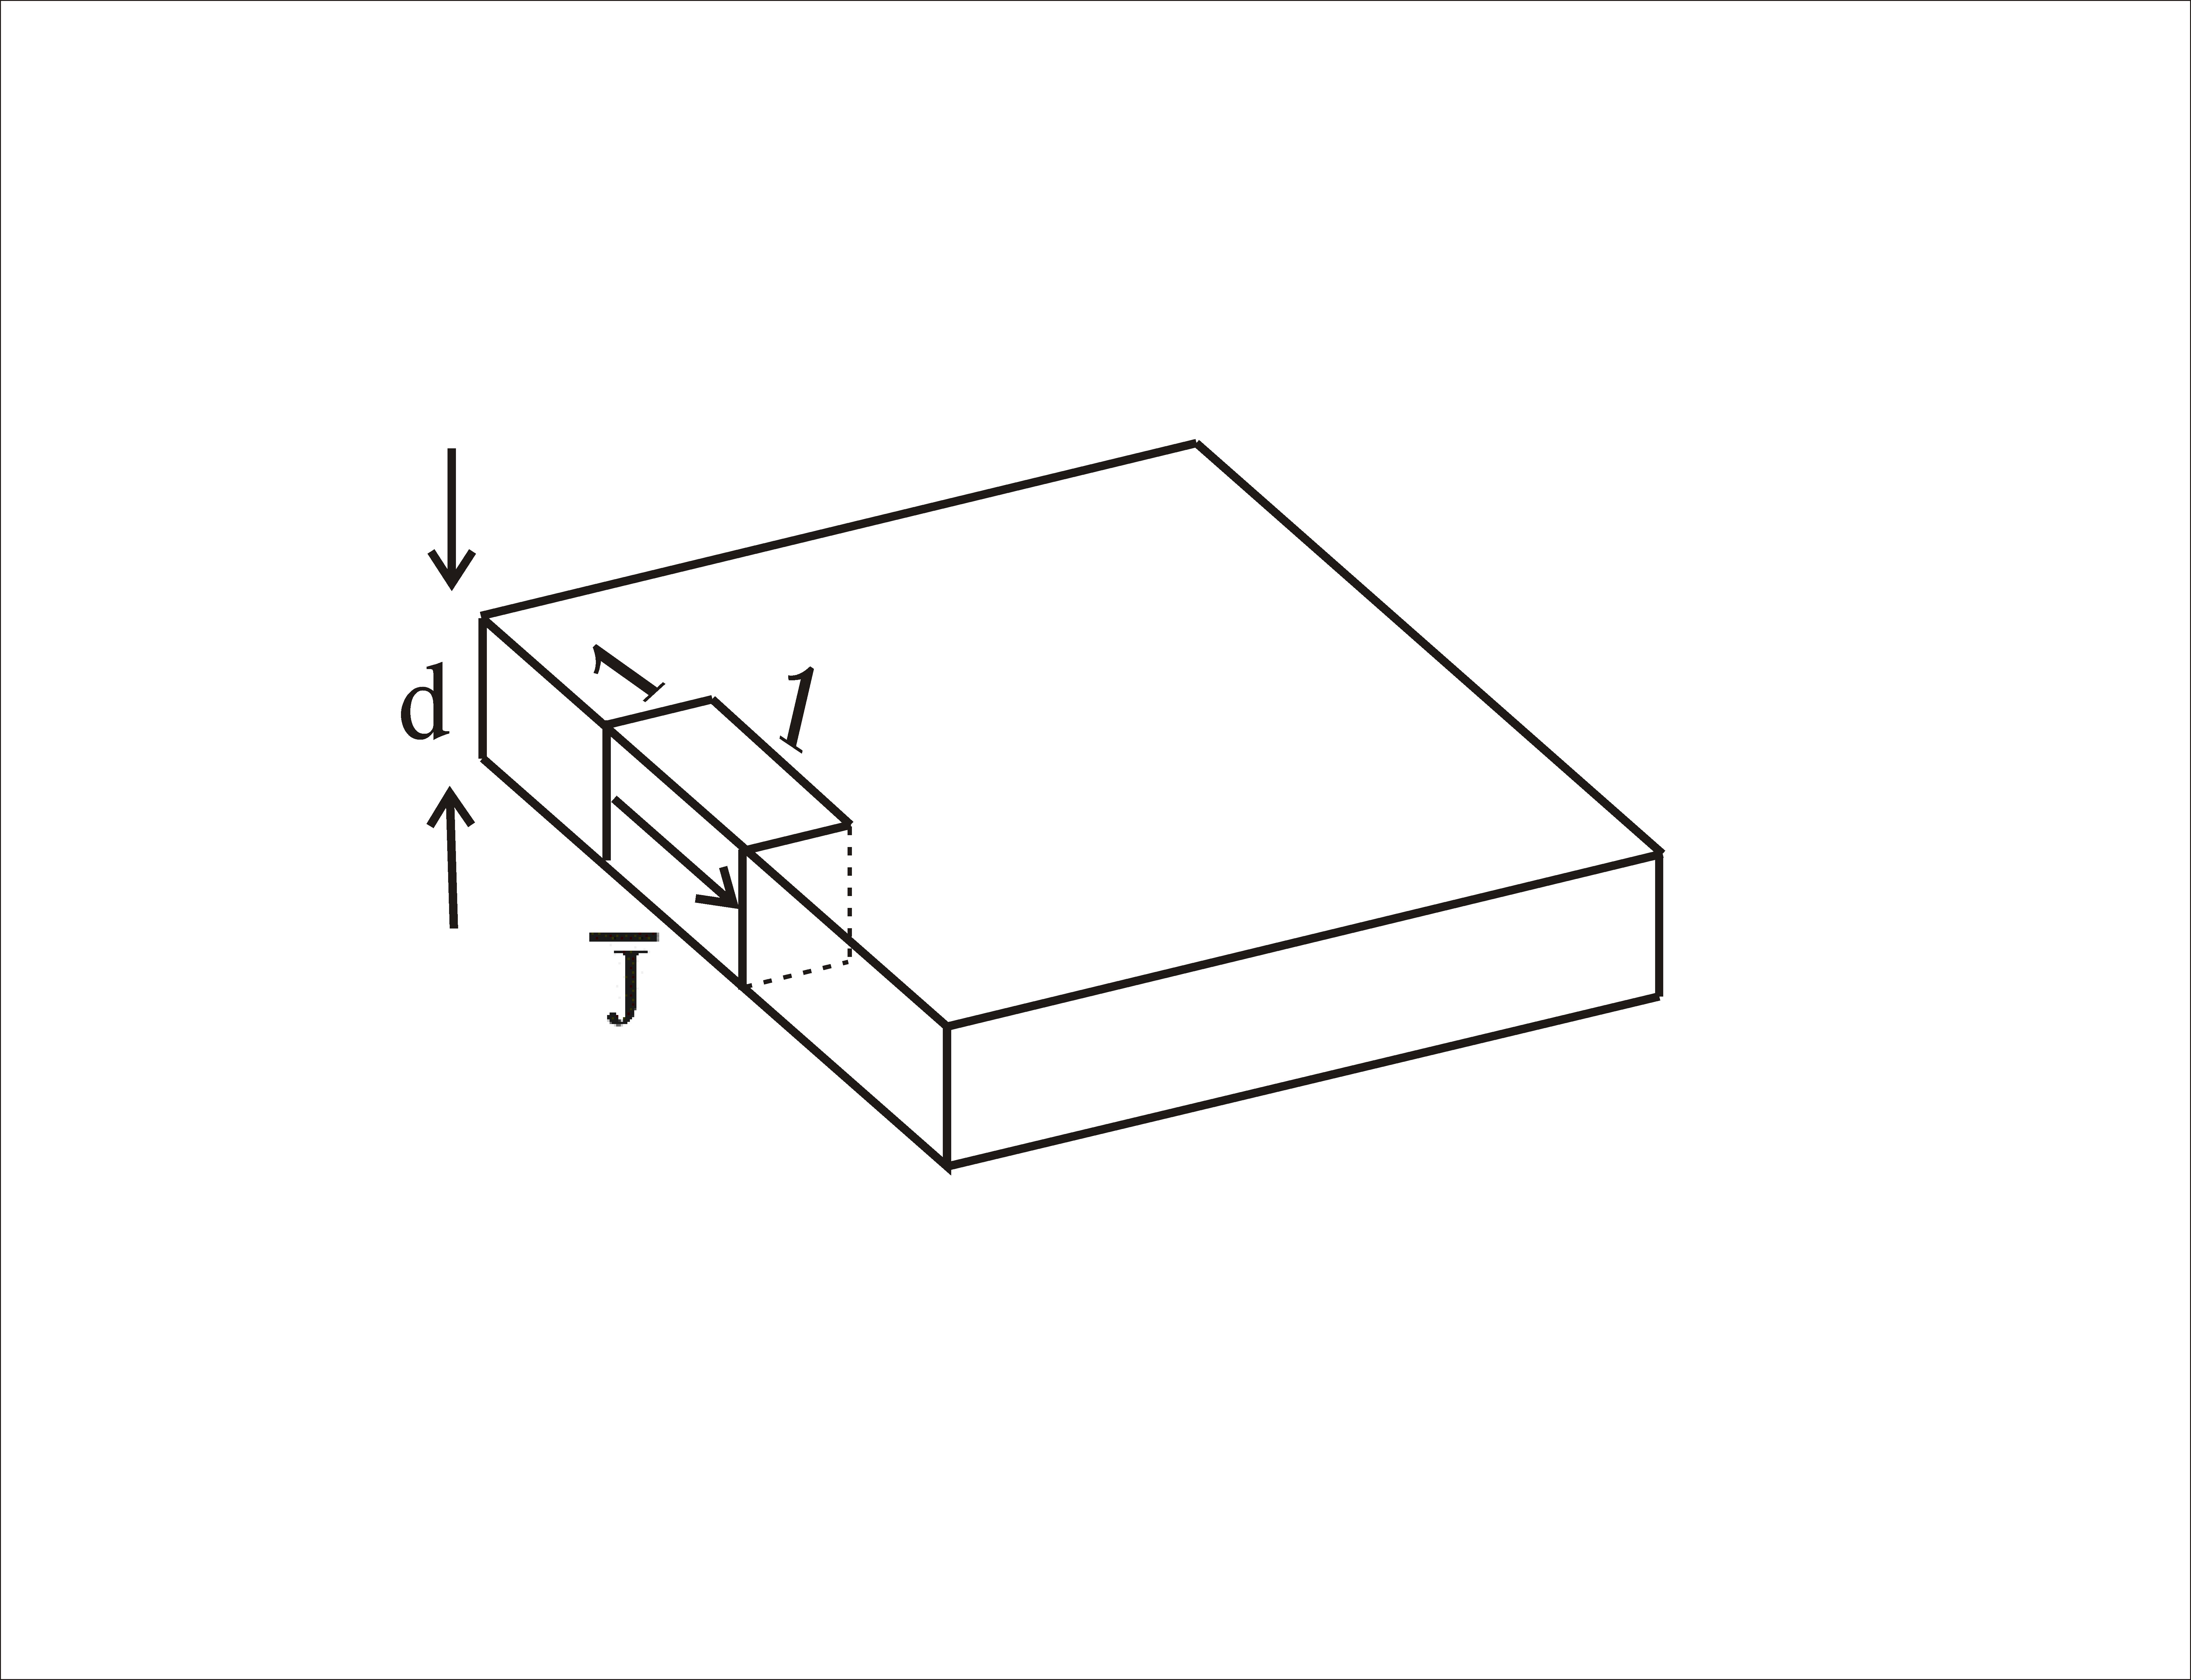
\includegraphics[width=1\linewidth]{surfacecurrent}
 	\caption{\textbf{Model for studying surface current}}
 \end{figure} 


 Lets say we have a slab of thickness d carrying current $\bar{J}$ as shown in figure 19.3. So the current flowing in the unit element is $\bar{J}\times$\{surface of the unit element through which $\bar{J}$ flows\} (note that '$\times$' represents multiplication not cross product).
 This surface considered through which $\bar{J}$ flows has its direction parallel to that of $\bar{J}$ and is shown by the dotted line.\\ 
 So we get that current flowing in the unit element is given by; $\bar{J}\times(d\times1)=\bar{J}d$. Again if we make $d\rightarrow0$ and $\bar{J}$ goes to infinity , you will have a current truly flowing on the surface and that current is the \textbf{surface current} $\bar{J}_{s}$. \\
 So essentially surface current is given by;
 \begin{align}
 \bar{J}_{s}=\lim_{d\rightarrow0}\{\bar{J}d\}
 \end{align}
 
 
 Again this apply to boundaries which are conducting boundaries, so when the conducting of the medium becomes infinite, then the current which is $\bar{J}=\sigma\bar{E}$ for a finite electric field becomes infinite and then you have what is called a 'surface current'. Since the unit of conduction current density $\bar{J}$ is $A/m^{2}$, the unit of surface current density is A/m($\bar{J}\times d$). That is the reason this quantity is also called the $linear$ $surface$ $current$ $density$ because it is defined per unit length.
 
 
 In all we are having quantities like charge density or volume charge density $\rho$, we have conduction current density $\bar{J}$, we have displacement current density $\frac{\partial\bar{D}}{\partial t}$, we have surface charge density$\rho_{s}$ and we have surface current density $\bar{J}_{s}$. Generally one will say that these are the sources which are related to the electric and magnetic fields. So one cn establish a relationship between these quantities which are the sources of the fields and these relationship are called \textbf{ boundary conditions}. Now let us solve some problems to reinforce these concepts.\\
 
 \section{Problems}
 \textbf{Problem 1};\\
 The volume charge density inside a hollow sphere is 
 \begin{align*}
 \rho=10e^{-20r} C/m^{3}.
 \end{align*}
 Find the total charge enclosed within the sphere. Also find the electric flux density on the surface of the sphere for radius of 2m.\\
 \textbf{Solution};\\
 \begin{figure}[h]
 	\centering
 	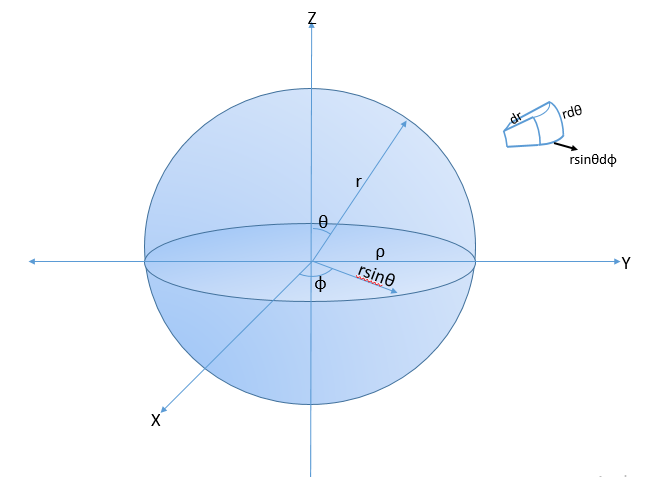
\includegraphics[width=1\linewidth]{fig194}
 	\caption{\textbf{spherical coordinate system}}
 \end{figure} 
 Total charge enclosed in the sphere is;
 \begin{center}
 	 \begin{align*}
 	Q=\iiint\limits_V\rho dv\\
 	\textbf{ from figure 19.4}, dv= dr\times(rsin\theta d\phi)\times rd\theta \\
 	dv=r^{2}sin\theta drd\theta d\phi\\
 	\textbf{so}, Q=\int^{2\pi}_{\phi=0}\int^{\pi}_{\theta=0}\int^{2}_{r=0} \rho r^{2}sin\theta drd\theta d\phi\\
 	Q= \int^{2\pi}_{\phi=0}d\phi\int^{\pi}_{\theta=0}sin\theta d\theta\int^{2}_{r=0}10e^{-20r}r^{2}dr
 	 \end{align*}
 \end{center}
 integrating this would give the value of Q and so we get that;
 \begin{align*}
 Q=\frac{\pi}{100} C
 \end{align*}
 To find the electric flux density, we use gauss lw which states that the electric flux density over the entire area of the sphere is equal to the total charge enclosed. Since the surface is  spherical, and the charges are distributed in a spherical symmetric manner, the electric displacement would be uniformly surface of the sphere. So we can find it according to gauss law.
\begin{align}
4\pi r^{2}D=Q=\frac{\pi}{100}\\
D=\frac{Q}{4\pi r^{2}}= 6.25\times10^{-4} C/m^{2}
\end{align}
 \\\\
 \textbf{Problem 2};\\
 The electric flux density is given as
 \begin{align*}
 \bar{D}=x^{3}\hat{x} + x^{2}y\hat{z}.
 \end{align*}
 Find the charge density inside a cube of side 2m placed at the origin with its side along the coordinate axes.\\
 \textbf{Solution};\\
 Here we use differential form of gauss law to find out first the charge density then the charge enclosed inside the cube.\\
 \begin{align*}
 \textbf{using gauss law}; \nabla\cdot\bar{D}=\rho\\
 \dfrac{\partial D_{x}}{\partial x}+\dfrac{\partial D_{y}}{\partial y}+\dfrac{\partial 
 D_{z}}{\partial z}=\rho \\
 \end{align*}
 substituting $\bar{D}$ components, we have;
 \begin{align*}
 \rho= \dfrac{\partial}{\partial x}(x^{3})+ 0 +\dfrac{\partial }{\partial z}(x^{2}y)\\
 \rho=3x^{2} .
 \end{align*}
 To get the total charge enclosed Q, we take the volume integral of the charge density $\rho$
 \begin{align*}
 Q=\int_{-1}^{1}\int_{-1}^{1}\int_{-1}^{1}\rho dxdydz, \\
 Q=\int_{-1}^{1}\int_{-1}^{1}\int_{-1}^{1}3x^{2}dxdydz \\
 Q=12\int_{-1}^{1}x^{2}dx= 12\frac{2}{3}
 Q= 8 C
  \end{align*}
 This could also be solved using the integral form of gauss law.\\
 \textbf{Problem 3};\\
  In a conducting medium the magnetic field is given as
  \begin{align*}
  \bar{H}=y^{2}z\hat{x}+2(x+1)yz\hat{y}-(x+1)z^{2}\hat{z}.
  \end{align*}
  Find the conduction current density at point (2,0,-1)m. Also find the current enclosed by a square loop y=1,  $0<x<1$, $0<z<1$.\\
   \textbf{Solution};\\
   \begin{figure}[h]
   	\centering
   	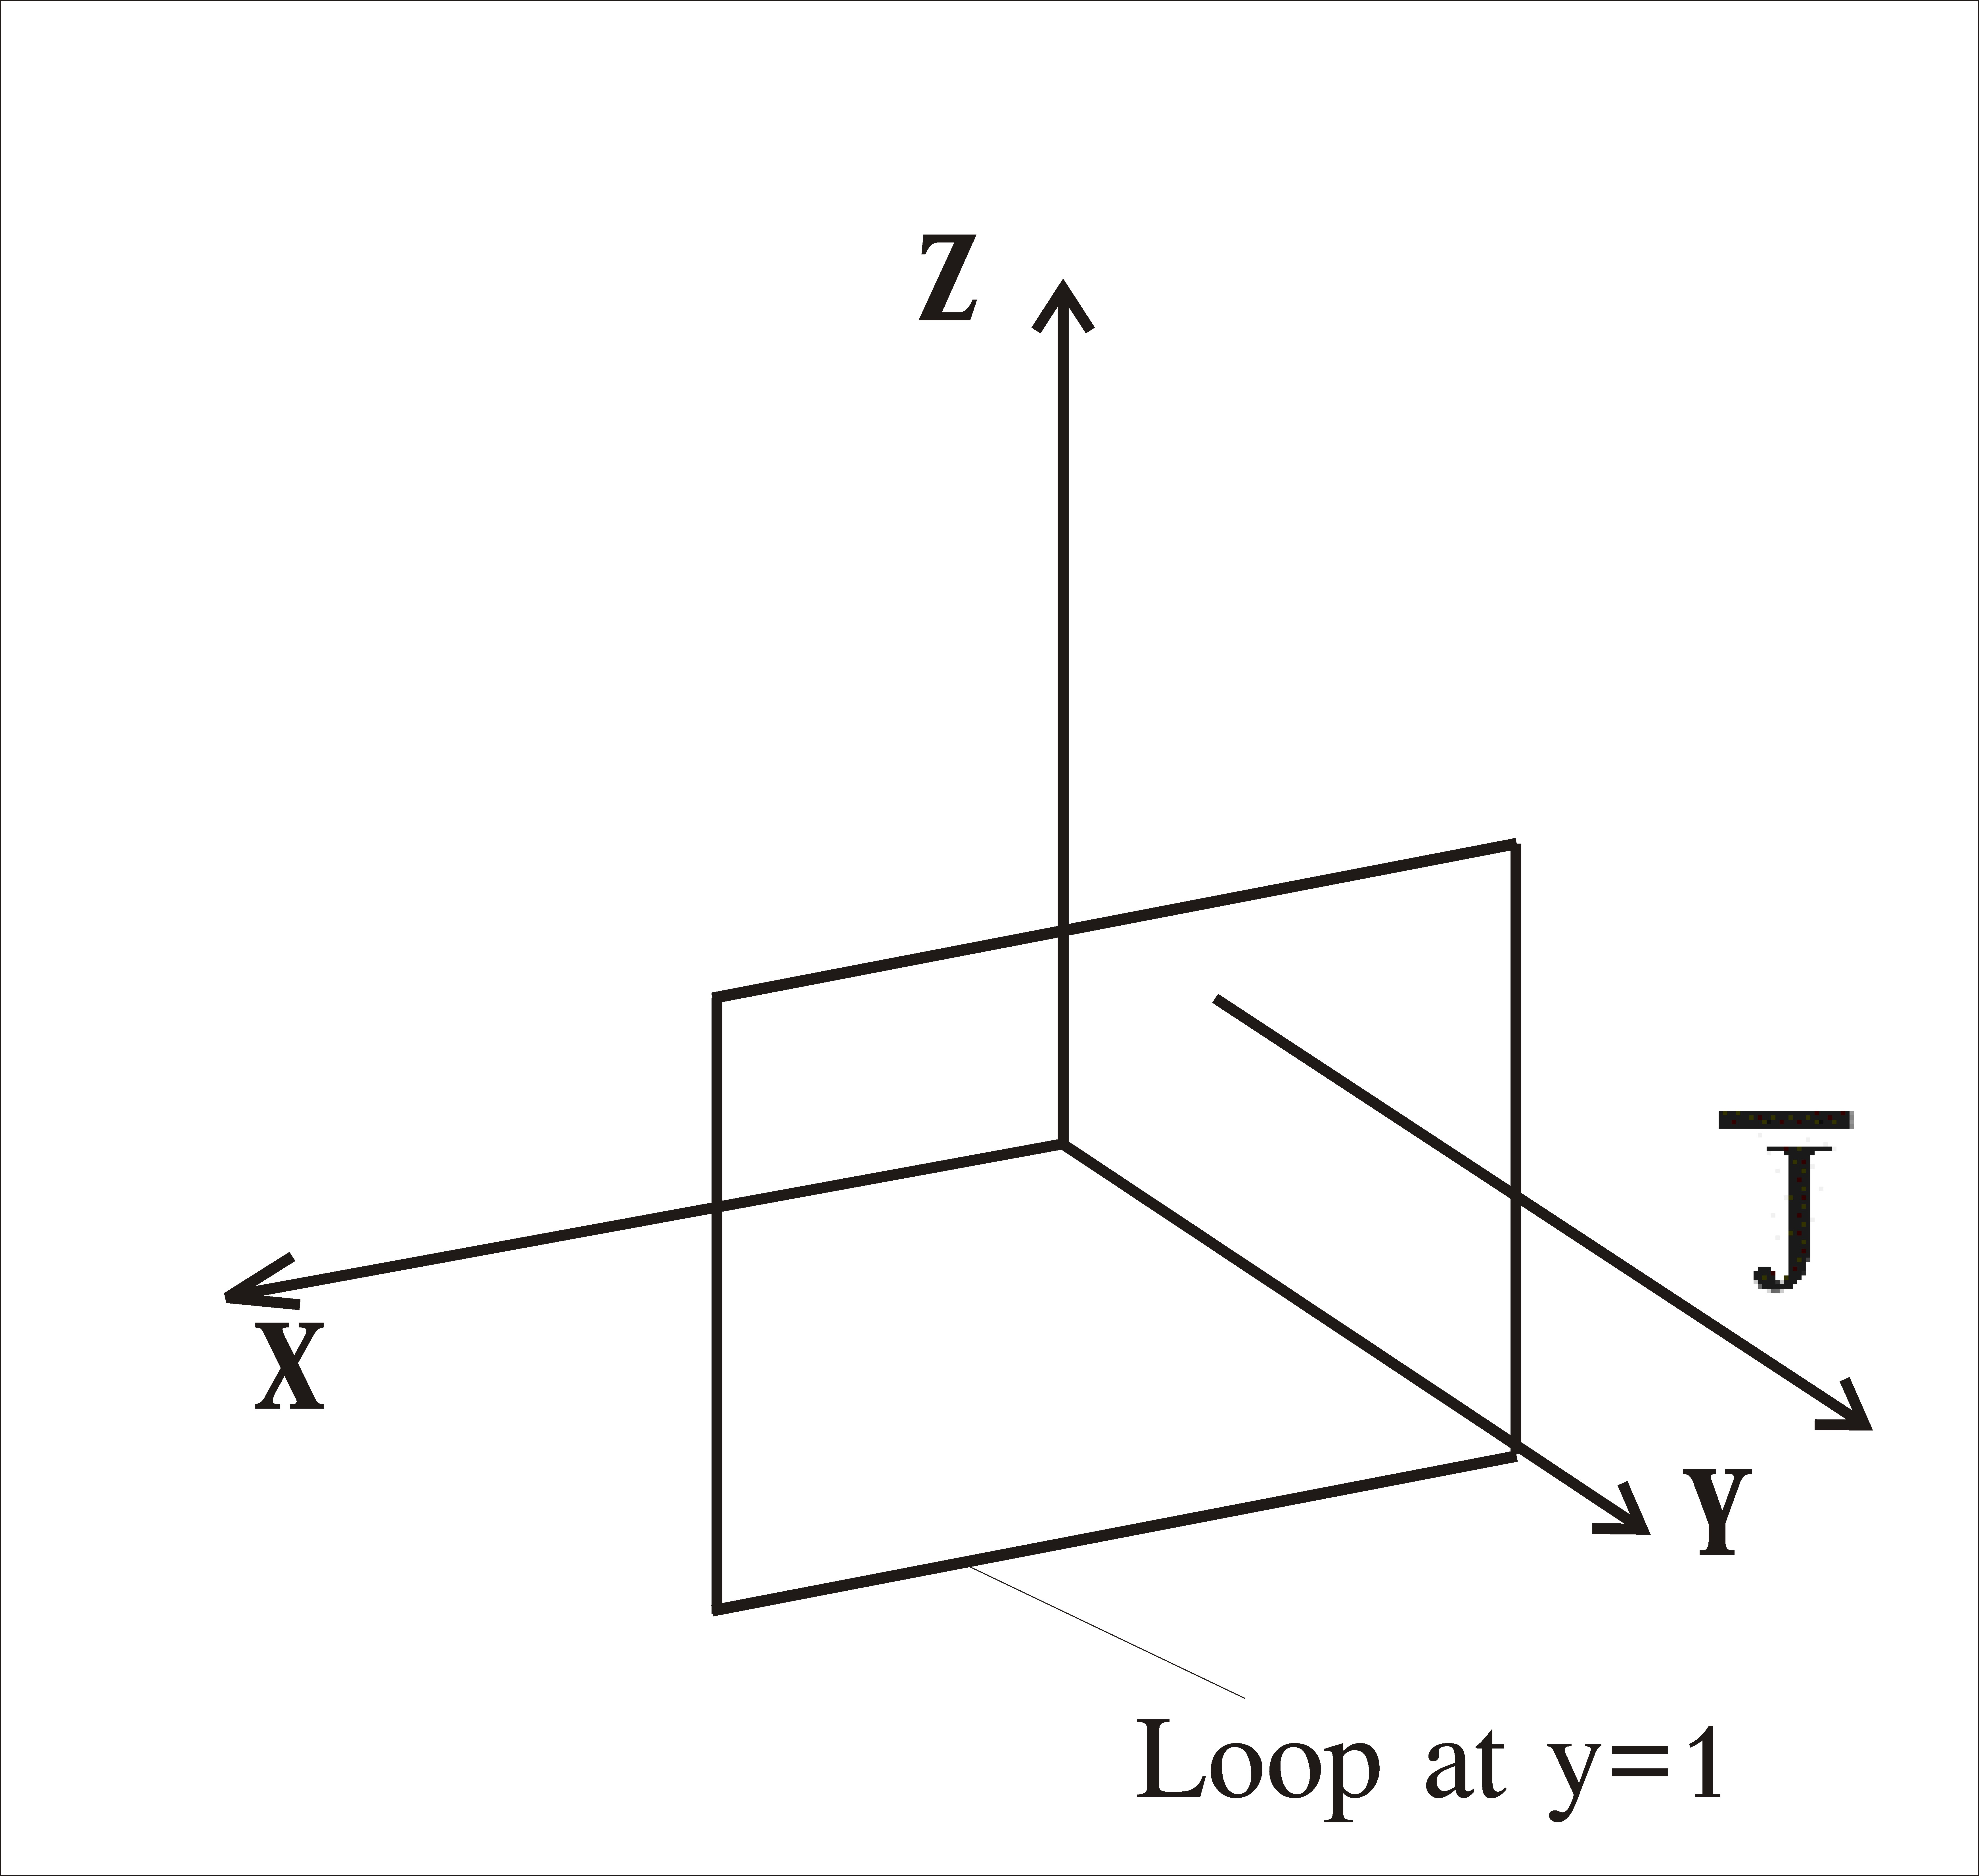
\includegraphics[scale=0.35]{problem3b}
   	\caption{\textbf{Loop at y=1}}
   \end{figure} 
   Here we will use amperes law(differential form) to solve for the conduction current density. Amperes law is given by;
   \begin{align*}
   \bar{J}=\nabla\times\bar{H}\\
    \end{align*}
    This is essentially the curl of $\bar{H}$ and is evaluated by solving for determinant of the matrix formed by $\nabla$ and $\bar{J}$ .\\
     so we have that $\bar{J} =$
    \[
    \left|
    \begin{tabular}{c c c}
    $\hat{x}$ & $\hat{y}$ & $\hat{z}$\\
    $\frac{\partial}{\partial x}$ &  $\frac{\partial}{\partial y}$ &  $\frac{\partial}{\partial z}$\\
    $H_{x}$ & $H_{y}$ & $H_{z}$
    \end{tabular}
    \right|
    \]
    
   \begin{align*}
  \bar{J}= (\frac{\partial H^{z}}{\partial y}-\frac{\partial H^{y}}{\partial z})\hat{x}+ (\frac{\partial H^{x}}{\partial z}-\frac{\partial H^{z}}{\partial x})\hat{y}+ (\frac{\partial H^{y}}{\partial x}-\frac{\partial H^{x}}{\partial y})\hat{z}\\\\
  \end{align*}
  Solving, we get;
   \begin{align*}
   \bar{J}=-2(x+1)y\hat{x}+(y^{2}+z^{2})\hat{y}
   \end{align*}
   At location (2,0,-1) the conduction current density is;
   \begin{align*}
   \bar{J}=\hat{y}
   \end{align*}
   
   With conduction current density $\bar{J}$ known, we can now find out the current enclosed by a loop at y=1 by integrating $\bar{J}$ over the area of the loop. The conduction current density is perpendicular to the plane created by that loop.
   
   \begin{figure}[h!]
   	\centering
   	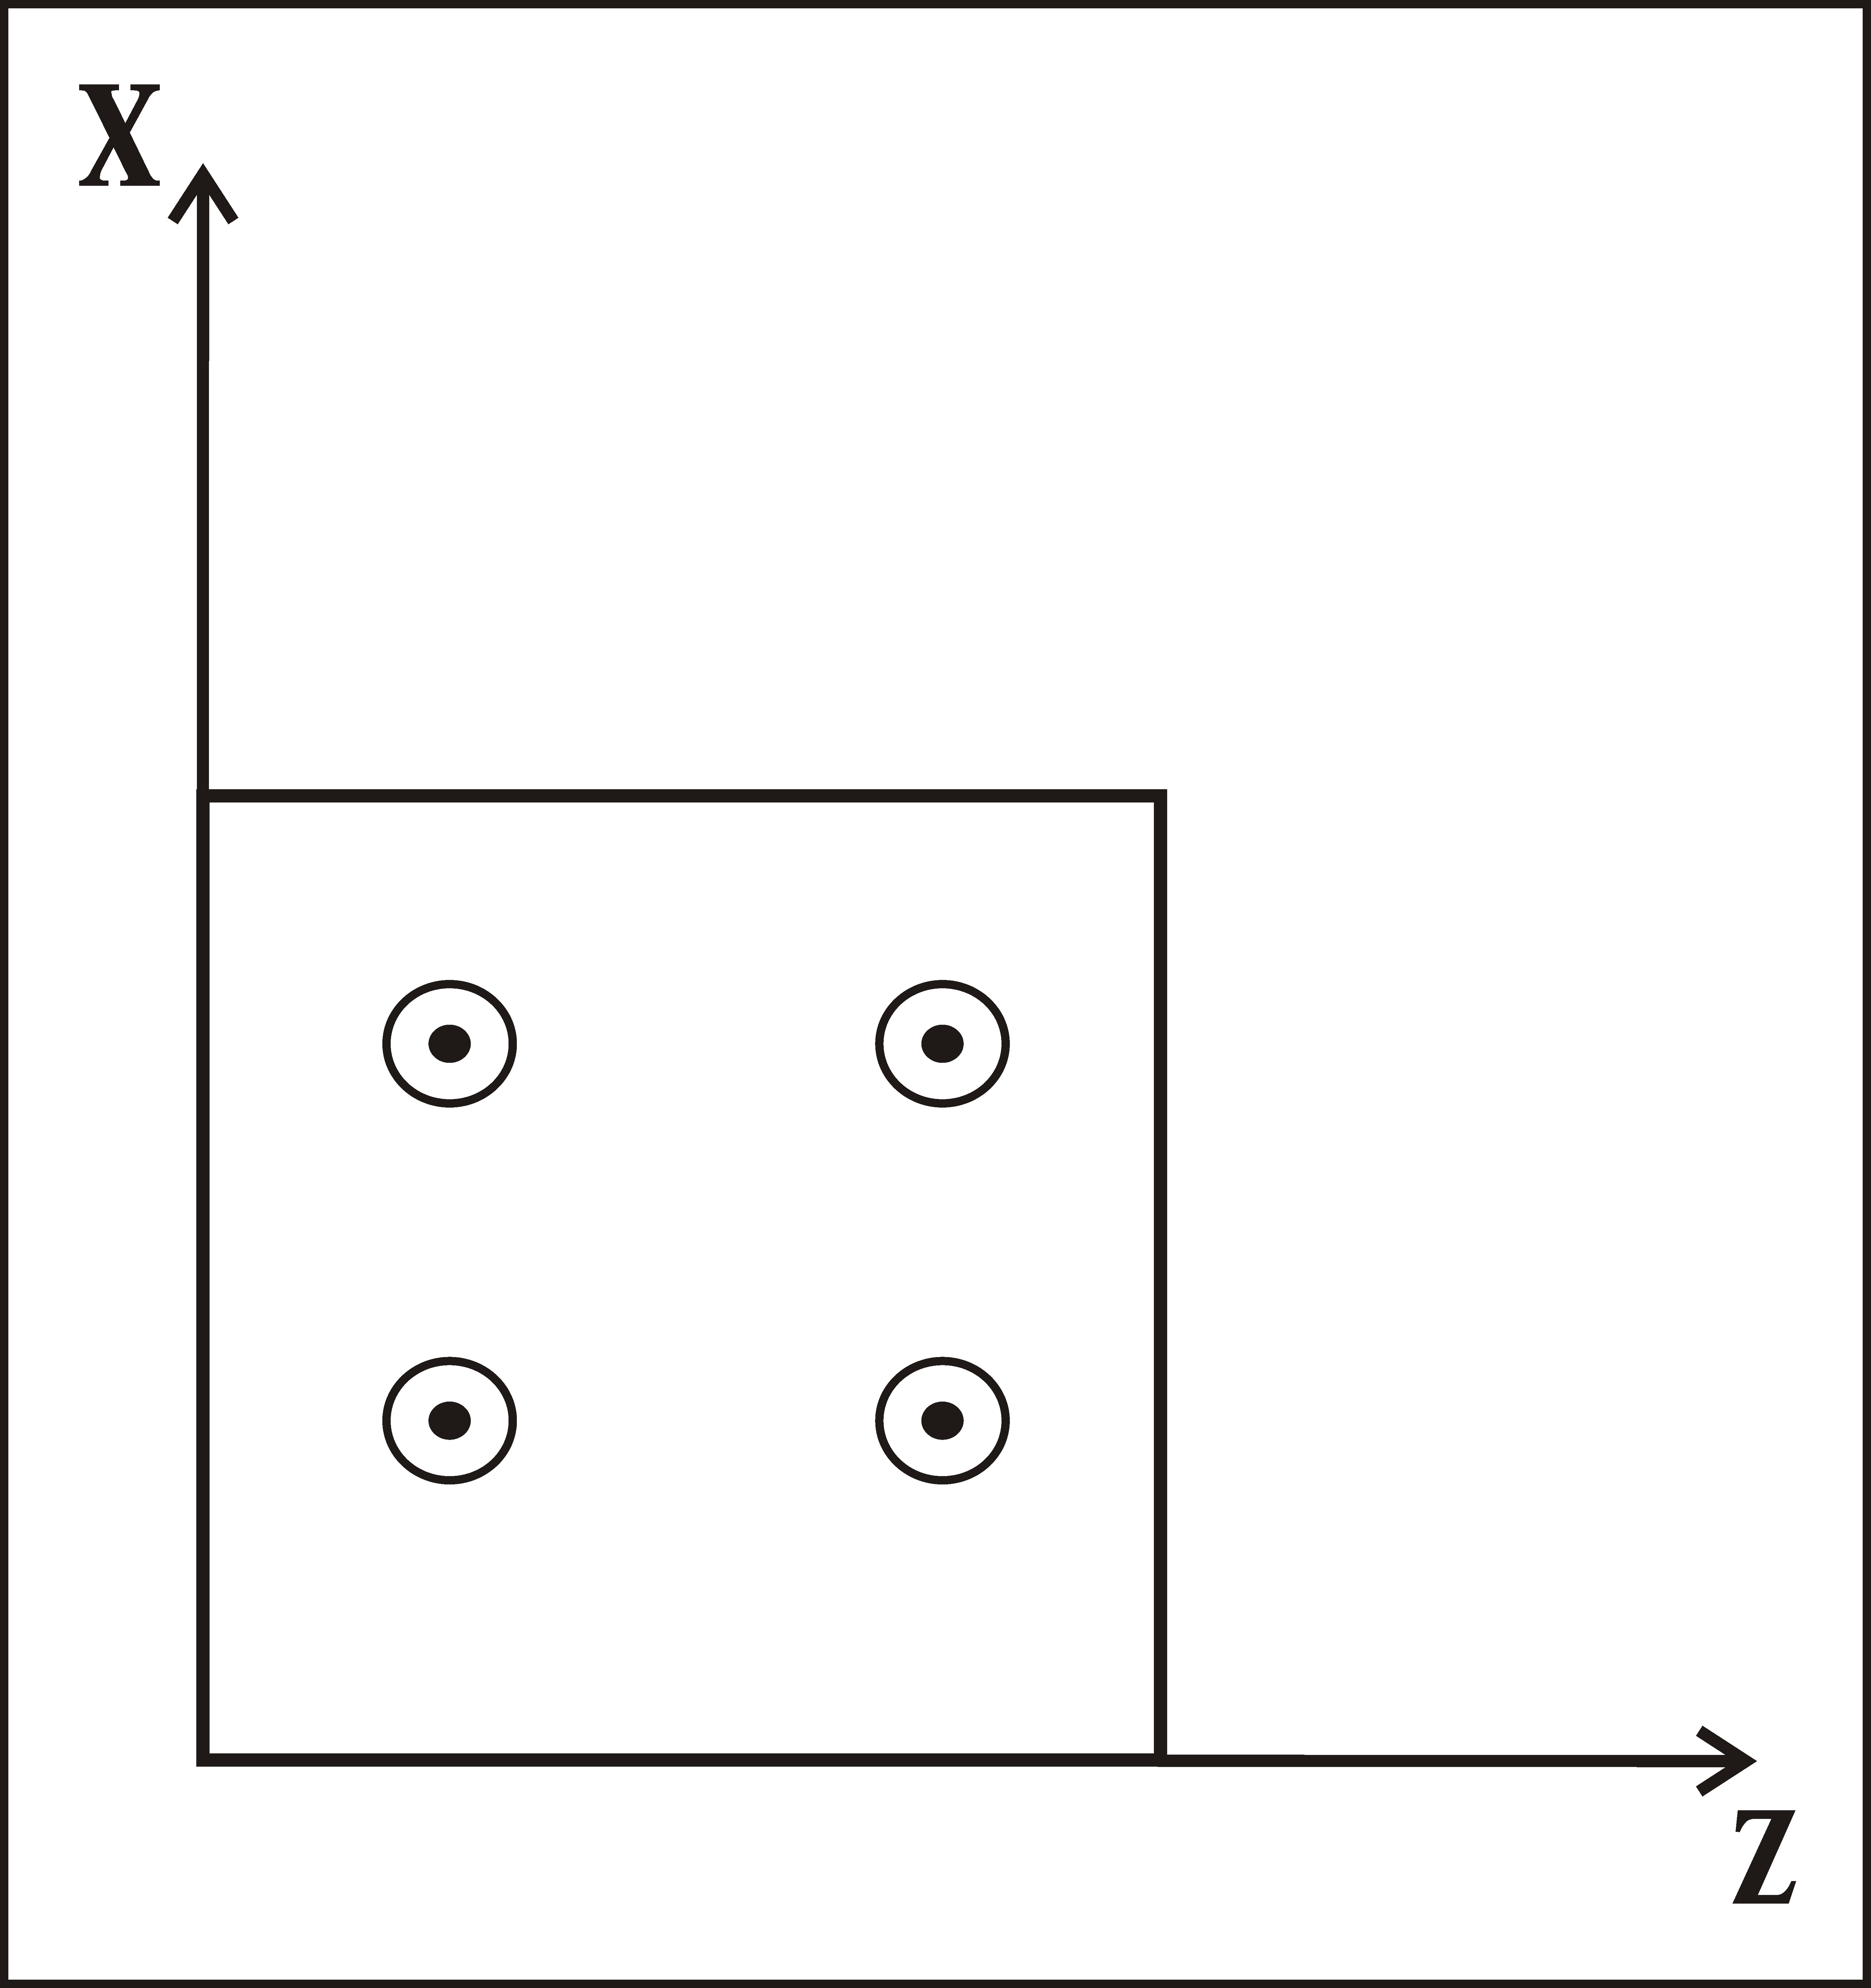
\includegraphics[scale=0.35]{problem3}
   	\caption{\textbf{Direction of conduction current in the XZ plane}}
   \end{figure} 
So looking in the XZ plane as shown in figure 19.6, if we go by the right hand rule, we have to go in anti-clockwise direction to get the current flowing in that direction(perpendicular to the plane created by the loop).
\begin{align*}
I=\iint\bar{J}\bar{da}=\iint\bar{J}\hat{y}dxdz\\
=\int_{0}^{1}\int_{0}^{1}J_{y}dxdz \\
=\int_{0}^{1}\int_{0}^{1}(y^{2}+z^{2})dxdz\\
\textbf{at} y=1\\
=\int_{0}^{1}\int_{0}^{1}(1+z^{2})dxdz\\
I= \frac{4}{3}A
\end{align*}
So these are some simple problems which essentially give you some feel on how to apply maxwell's equations in real life, either with the differential form or integral form.